\documentclass[journal]{IEEEtran}

\ifCLASSINFOpdf

\else

\fi

\hyphenation{op-tical net-works semi-conduc-tor}
\usepackage{amsmath}
\usepackage{graphicx} 
\usepackage{appendix} 
\usepackage{float}


\begin{document}

\title{BantayLaot: Fish Catch Documentation and IUU Fishing Monitoring for Municipal Fisheries in the Philippines Using Mobile and Web Technologies}


\author{Jose~Benjamin~Gallero~\IEEEmembership
        and~Val~Randolf~M.~Madrid~\IEEEmembership% <-this % stops a space
}

\markboth{CMSC 190 SPECIAL PROBLEM, INSTITUTE OF COMPUTER SCIENCE}%
{Shell \MakeLowercase{\textit{et al.}}: Bare Demo of IEEEtran.cls for IEEE Journals}

\maketitle
\begin{abstract}
Illegal, unreported, and unregulated (IUU) fishing threatens the sustainability of municipal fisheries in the Philippines. BantayLaot, a mobile and web-based Vessel Monitoring System (VMS), addresses this issue by leveraging GPS-enabled mobile devices for asynchronous vessel tracking, fish catch documentation, and IUU violation reporting. Developed using Kotlin and the MERN stack, the system provides geospatial visualization, CPUE analysis, and offline data collection for limited-connectivity areas. BantayLaot offers a scalable and cost-effective solution to improve fisheries management and promote sustainable practices.
\end{abstract}

\begin{IEEEkeywords}
IUU, VMS, Fish Catch Documentation.
\end{IEEEkeywords}

\IEEEpeerreviewmaketitle

\section{Introduction}
\IEEEPARstart 
The Philippines has a rich maritime heritage and contains enormous marine resources that have historically ensured the livelihoods of millions of Filipinos. Nevertheless, the sector faces significant challenges, compounded by illegal, unreported, and unregulated (IUU) fishing activities, as well as persistent difficulties in the governance and regulation of fisheries in the Philippines. Despite its considerable contributions to economic growth and food security, the fisheries sector continues to struggle against these issues. A joint report by the Philippine Bureau of Fisheries and Aquatic Resources (BFAR) and the United States Agency for International Development (USAID) in 2021 estimated annual losses of ₱62 billion due to IUU fishing. The report also revealed that approximately 30 percent of municipal vessels, equating to 30,000 boats, remain unregistered, while vessels identified as commercial fail to report up to 422,000 metric tons of fish annually. These IUU fishing activities not only undermine the sustainability of marine ecosystems but also deprive coastal communities of vital income opportunities.

The significance of the fisheries sector to the Philippine economy cannot be overstated. Despite its relatively modest contribution of 12.82\% to the country's Gross Value Added (GVA), fisheries provide livelihoods for approximately 2.3 million fisherfolk, representing 5\% of the labor force. Moreover, fisheries contribute to 11.68\% of the food consumption of Filipinos, particularly benefiting those reliant on subsistence fishing for sustenance. Alarmingly, fisherfolk, alongside farmers, children, and rural inhabitants, remain among the most marginalized segments of society. According to the Philippine Statistics Authority (PSA, 2023), poverty rates among fisherfolk have surged to 30.6\%, reflecting an ongoing and distressing trend of increasing deprivation within these vulnerable communities.

This research introduces BantayLaot, a Vessel Monitoring System (VMS) leveraging mobile and web technologies to address these challenges. BantayLaot is designed to revolutionize fish catch documentation and IUU fishing monitoring in municipal fisheries by using fishermen's mobile phones as transceivers. Inspired by successful implementations in other maritime nations, BantayLaot provides a cost-effective and accessible solution. By harnessing geospatial data, automated documentation, and data analytics, BantayLaot seeks to enhance regulation and support sustainable fishing practices, ultimately safeguarding marine resources and fostering economic growth in the Philippines.


\subsection{Statement of the Problem}
The US Agency for International Development and the Bureau of Fisheries and Aquatic Resources have reported that IUU fishing poses a serious threat to the sustainability of municipal fisheries in the Philippines. It exacerbates economic losses and undermines the livelihoods of coastal communities. Existing regulatory frameworks and enforcement mechanisms remain insufficient in addressing these challenges, highlighting the need for innovative solutions to enhance monitoring and surveillance efforts.

\subsection{Objectives of the Study}
This study aims to develop and evaluate BantayLaot, a VMS and fish catch documentation tool designed to combat IUU fishing in municipal fisheries across the Philippines while promoting sustainable fishing practices. Specifically, the study seeks to:
\begin{enumerate}
    \item Develop BantayLaot as a VMS for tracking municipal fishing vessels;
    \item Implement fish catch documentation features;
    \item Implement an IUU reporting feature with geotagged location data; and
    \item Provide data visualization capabilities on BantayLaot's web platform.
\end{enumerate}

\subsection{Significance of the Study}
The development and implementation of BantayLaot as a Vessel Monitoring System (VMS) and fish catch documentation tool offer significant benefits to various stakeholders, including fisherfolk, government agencies, researchers, conservationists, and industry players. The system enhances transparency, accountability, and regulatory enforcement by providing data on fishing activities. This supports sustainable practices and evidence-based decision-making. Furthermore, BantayLaot promotes data transparency and interoperability, enabling scientific research and policy analysis. Ultimately, the system addresses the challenges of IUU fishing and fish catch documentation, contributing to the long-term sustainability of coastal communities, marine ecosystems, and the fisheries sector in the Philippines.


\subsection{Scope and Limitations}

This study focuses on the development and implementation of BantayLaot, a Vessel Monitoring System (VMS) and fish catch documentation tool aimed at addressing illegal, unreported, and unregulated (IUU) fishing in the Philippines. The system consists of a mobile application for fishermen, providing GPS-based vessel tracking, fish catch documentation, and offline data collection, alongside a web platform for stakeholders to visualize and analyze fishing data.

The project is limited by its reliance on internet connectivity for data synchronization, which may delay real-time updates in areas with poor connectivity. GPS accuracy and mobile device battery consumption are also potential constraints. Furthermore, the system was not tested in actual fishing conditions; dummy data was used for testing and demonstration. This limitation affects the assessment of the system’s practical effectiveness in real-world scenarios. Despite these constraints, BantayLaot provides a foundation for enhancing municipal fisheries management and can be iteratively improved through future field testing and technology integration.

\section{Review of Literature}
\subsection{Mobile Application Technological Framework}
For the development of the mobile platform of BantayLaot, the chosen primary approach is Native Android, particularly Kotlin. This choice provided optimal performance, efficient power management, and full access to the features of an Android mobile device, particularly the embedded GPS, which is essential for tracking and reporting municipal fishing vessels. Native Android development, using Java and Kotlin, is known for its performance and optimization of device resources. Comparative studies, such as those by Hussain et al. (2021), have shown that native apps outperform cross-platform frameworks like Flutter in terms of CPU consumption, memory usage, and responsiveness. Native development ensure access to the latest Android APIs and tools, allowing BantayLaot to utilize cutting-edge features and security enhancements.

Kotlin offers significant advantages over Java, making it a preferable option for developing BantayLaot’s mobile platform. Studies, such as those by Ardito et al. (2020), indicate that Kotlin reduces the lines of code and minimizes the chances of errors, thus making the development process more manageable. Kotlin's null safety feature helps prevent errors related to nullable data types, ensuring system stability and reliability. Additionally, Kotlin's interoperability with Java guarantee compatibility with MongoDB Java drivers, facilitating data exchange between the mobile platform and the MongoDB database (Fotache \& Cogean, 2013). This compatibility is crucial for the efficient functioning of the BantayLaot system.

Moreover, Kotlin's ability to integrate seamlessly with existing Java codebases ensures that the transition to this newer language can be smooth and efficient. The BantayLaot mobile platform leverages these capabilities to create a robust application that can handle real-time data collection and processing efficiently. Ensuring optimal battery usage while maintaining accuracy is another critical consideration for the development. By employing best practices in Kotlin and utilizing the Android framework's capabilities, BantayLaot aims to deliver a high-performance mobile application that meets the stringent requirements of real-time vessel monitoring and data reporting.

\subsection{Web Platform Technological Framework}
The development of BantayLaot’s web platform utilizes the MERN stack, comprising MongoDB, Express.js, React, and Node.js. This stack is highly effective for dynamic web applications, offering efficiency, scalability, and seamless interaction between the front-end and back-end components.

MongoDB serves as a flexible and scalable NoSQL database, capable of handling large volumes of data in a JSON-like format. Its ability to manage unstructured or semi-structured data, along with horizontal scaling capabilities, makes it ideal for applications requiring dynamic and evolving data structures (Baid \& Gupta, 2024). MongoDB's schema-less nature allows for easy adaptation as data requirements change over time (Bawane et al., 2022).

Express.js acts as the server-side framework, simplifying the development of robust and scalable server applications. It provides essential functionalities and middleware support for processing HTTP requests and responses, enabling clean model-view-controller (MVC) architecture and rapid API endpoint development (Baid \& Gupta, 2024; Bawane et al., 2022).

React, the front-end library developed by Facebook, is known for its declarative and efficient approach to building user interfaces. React promotes a component-based architecture, allowing developers to create modular and reusable UI components, which enhances code maintainability and scalability (Baid \& Gupta, 2024). The implementation of the virtual DOM in React improves performance by efficiently updating and rendering components, ensuring a seamless user experience in single-page applications (Bawane et al., 2022).

Node.js serves as the JavaScript runtime environment, unifying the language across the MERN stack and allowing developers to use JavaScript for both front-end and back-end development. Its event-driven, non-blocking I/O model makes it lightweight and efficient, suitable for data-intensive real-time applications (Baid \& Gupta, 2024; Bawane et al., 2022).

The integration of these components through the MERN stack offers significant advantages in web development. The commitment to full-stack JavaScript enables seamless collaboration between front-end and back-end teams, promoting code consistency and reducing the learning curve (Baid \& Gupta, 2024). Additionally, the stack benefits from a robust community that provides ongoing support, a wealth of libraries, and readily available solutions to common development challenges.

By leveraging the MERN stack, BantayLaot's web platform achieves high performance and scalability, essential for handling the complex requirements of fisheries management and monitoring. The stack's suitability for handling asynchronous operations and real-time data makes it an ideal choice for applications requiring efficient data processing and user interactivity.

\subsection{Vessel Monitoring System (VMS)}
BantayLaot is implemented as a VMS, utilizing mobile technology to monitor fishing vessels. The system compiles and link fishing vessel positional data with catch records, allowing the creation of detailed spatial distribution maps of catch and fishing efforts. This combination is essential for accurate catch per unit effort (CPUE) estimates, providing critical information for fish stock management (Gerritsen \& Lordan, 2011). These features aims to curb illegal, unreported, and unregulated (IUU) fishing activities, a significant problem in the Philippines (Soemarmi et al., 2020).

The study by Soemarmi et al. (2020) in Indonesia highlights the effectiveness of VMS in enhancing monitoring and surveillance efforts, thereby reducing IUU fishing occurrences. Unlike hardware-dependent systems like the Integrated Marine Environment Monitoring System (IMEMS) developed by BFAR, BantayLaot leverages mobile technology for data collection, making it a more accessible and cost-effective solution. The integration of data with official databases streamlines the enforcement of fishing laws, allowing authorities to track and spot infractions instantly, thus promoting sustainable fishing methods and regulatory compliance.

Furthermore, BantayLaot's mobile-based approach allows for a more flexible and scalable implementation. This method is particularly advantageous for municipal fisheries, where resources may be limited, and the cost of dedicated hardware can be prohibitive. By using fishermen's mobile phones as transceivers, BantayLaot not only reduces costs but also simplify the deployment process. The use of mobile technology also facilitates the rapid adoption of the system, as it leverages devices that fishermen are already familiar with. This approach ensures that the system can be widely implemented across various regions, enhancing the overall effectiveness of fisheries management.
\subsection{Fish Catch Documentation System}
BantayLaot's fish catch documentation system streamlines data input and enhance the accuracy of catch records. Fishermen can log their daily catches using the BantayLaot smartphone application, which will timestamp and link data, including species, amount, and position, to the GPS coordinates of the vessel. This integration ensures that catch data is accurately synchronized with the vessel’s location using the Unix timestamp reference (Wahab et al., 2021). The recorded data is transmitted to the BantayLaot web platform, where it is aggregated and stored in a centralized database, ensuring data integrity and accessibility.

The documentation system features a user-friendly interface designed with input from potential end users. Using iconography, minimal text, and multilingual support, the system is accessible to fishermen with varying levels of technological literacy (Calderwood, 2022). Resources is available to educate users on the value of documentation and provide guidance on maximizing the system's potential. Effective fish catch documentation combined with vessel monitoring can significantly improve fisheries management and promote sustainable fishing methods.

The research by Wahab et al. (2021) on synchronizing fish catch data with VMS and the study by Gerritsen and Lordan (2011) on integrating VMS data with daily logbook records inspire this approach. These studies emphasize the importance of detailed insights into spatial patterns of catch distribution and fishing effort. By leveraging mobile technology, BantayLaot offers an accessible and cost-effective solution that is easier to implement compared to hardware-dependent systems like IMEMS. This approach helps ensure the long-term viability of coastal communities and the sustainability of marine ecosystems.

Additionally, the integration of a robust data synchronization mechanism is crucial for the success of the fish catch documentation system. Ensuring that catch data and corresponding GPS data are accurately linked is achieved through the use of the Unix timestamp, which guarantees precise and dependable data collection. This system facilitates asynchronous vessel surveillance and comprehensive fish catch documentation, aiding in the development of sustainable fishing practices and improving the livelihood of municipal fishermen in the Philippines.

\section{Methodology}

\subsection{Technology}
The BantayLaot mobile application and web platform were developed using the following specifications:
\begin{enumerate}
    \item \textbf{Operating System:} macOS Sequoia
    \item \textbf{Processor:} Apple M2
    \item \textbf{Memory:} 16GB LPDDR5 SDRAM
\end{enumerate}

\subsection{Development Tools}
The following tools and technologies were utilized during the development:
\begin{enumerate}
    \item \textbf{Visual Studio Code:} Used for developing the web platform.
    \item \textbf{Android Studio:} Utilized for mobile app development, testing, and debugging.
    \item \textbf{MERN Stack:} Includes MongoDB for data storage, Express.js for the back-end framework, React.js for the front-end interface, and Node.js for server-side processing.
    \item \textbf{Kotlin:} Used for building the mobile application, leveraging Jetpack Compose for modern and declarative UI development.
    \item \textbf{Leaflet and OpenStreetMap:} Used in the web application for interactive maps.
\end{enumerate}

\subsection{Use Case Scenarios}
The BantayLaot system encompasses two main components: a mobile application and a web-based platform. Each serves distinct but complementary roles in achieving the system's objectives.

\subsubsection{Mobile Application Use Case}
The mobile application is primarily used by fishermen at sea for data collection. Its functionalities include:
\begin{itemize}
    \item \textbf{GPS Tracking:} Continuous recording of location data during fishing sessions.
    \item \textbf{Catch Reporting:} Documentation of fish species, total catch weight, and fishing gear used.
    \item \textbf{Violation Reporting:} Capturing and uploading IUU (Illegal, Unreported, and Unregulated) fishing incidents with geotagged images.
    \item \textbf{Offline Mode:} Data is stored locally when offline and uploaded to the database upon reestablishing a connection.
\end{itemize}

\begin{figure} [H]%
    \centering
    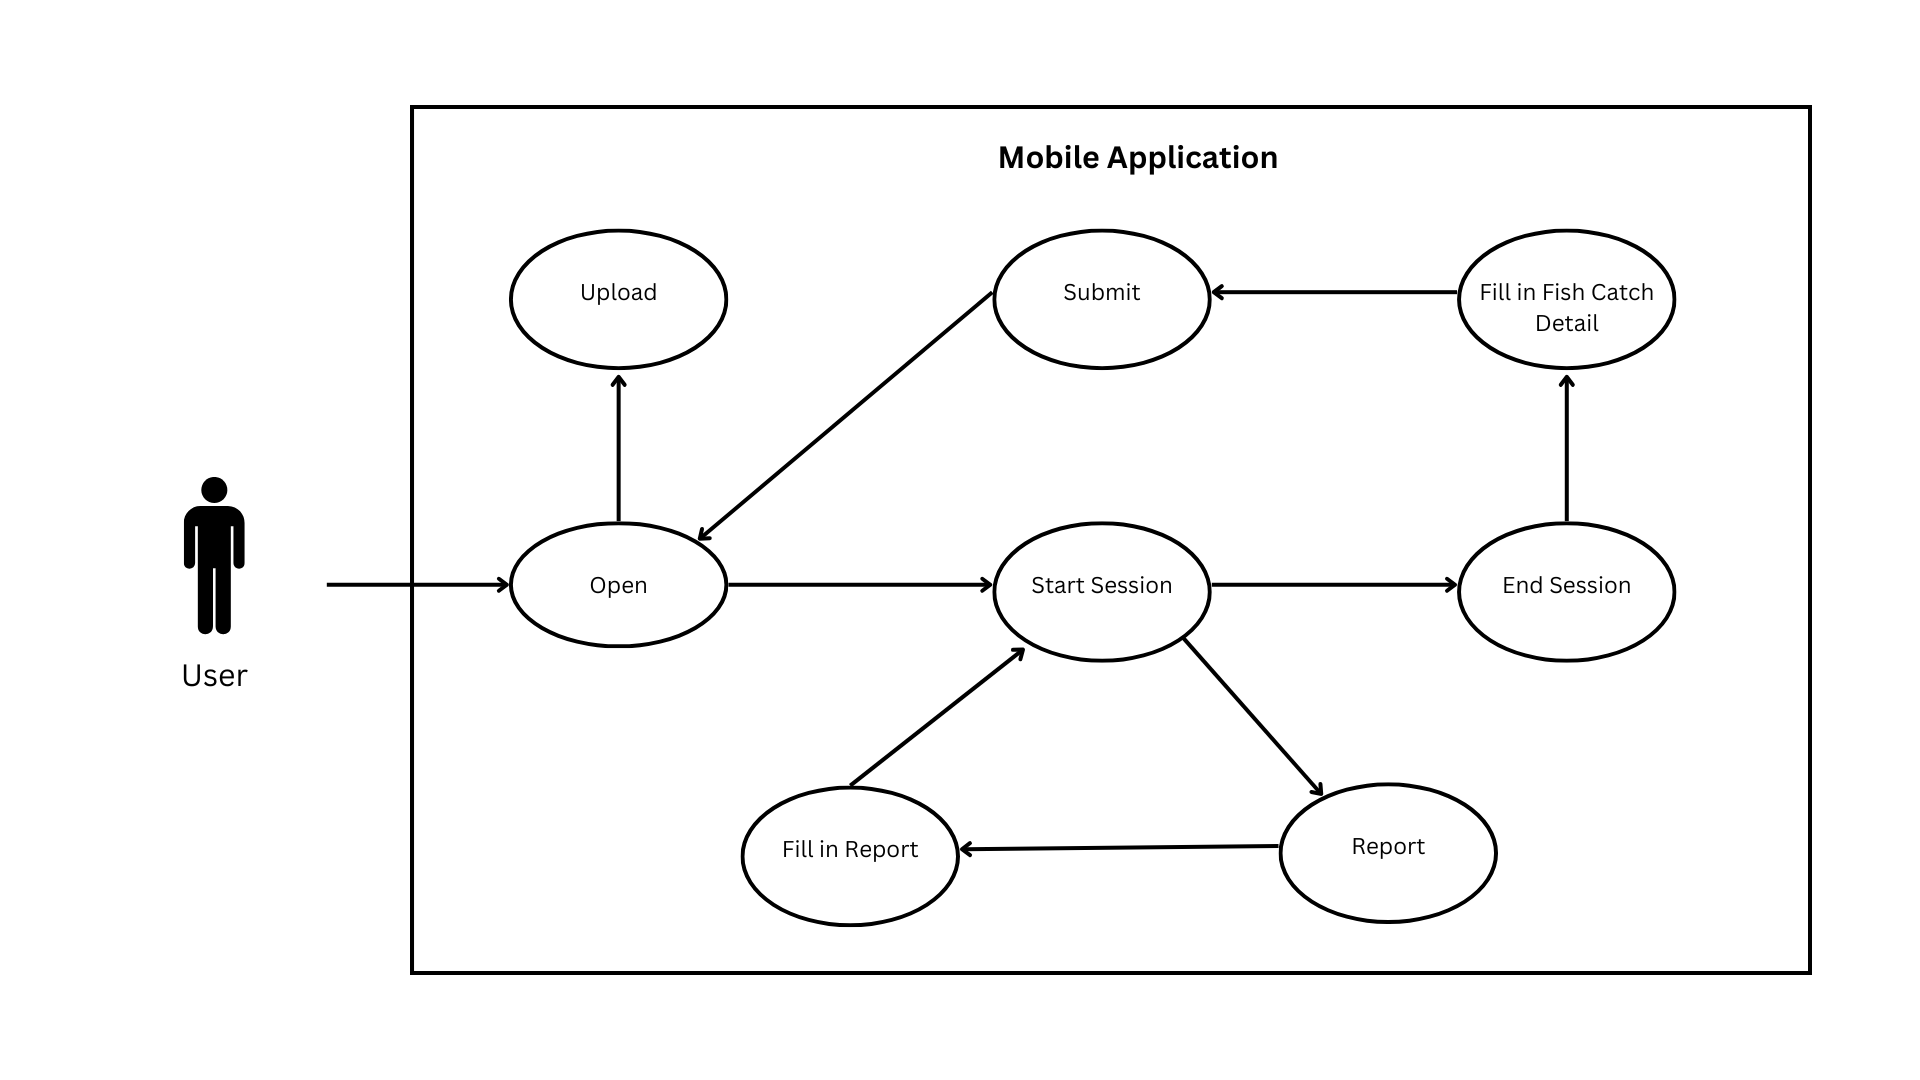
\includegraphics[width=1\linewidth]{Figure_1.png}
    \caption{Use Case Diagram for the Web Platform}
    \label{fig:enter-label}
\end{figure}


\subsubsection{Web Application Use Case}
The web-based platform is designed for monitoring and analysis by stakeholders, such as regulators or researchers. Its key functionalities include:
\begin{itemize}
    \item \textbf{Visualization:} Interactive maps displaying fishing session routes and IUU violation reports.
    \item \textbf{Analysis:} Aggregated metrics, such as Catch Per Unit Effort (CPUE), and summary charts for decision-making.
    \item \textbf{Violation Monitoring:} Temporal and spatial trend analysis of reported violations.
    \item \textbf{Filtering and Reporting:} Capability to filter data by vessel, date, or gear type for targeted investigations.
\end{itemize}

\begin{figure} [H]%
    \centering
    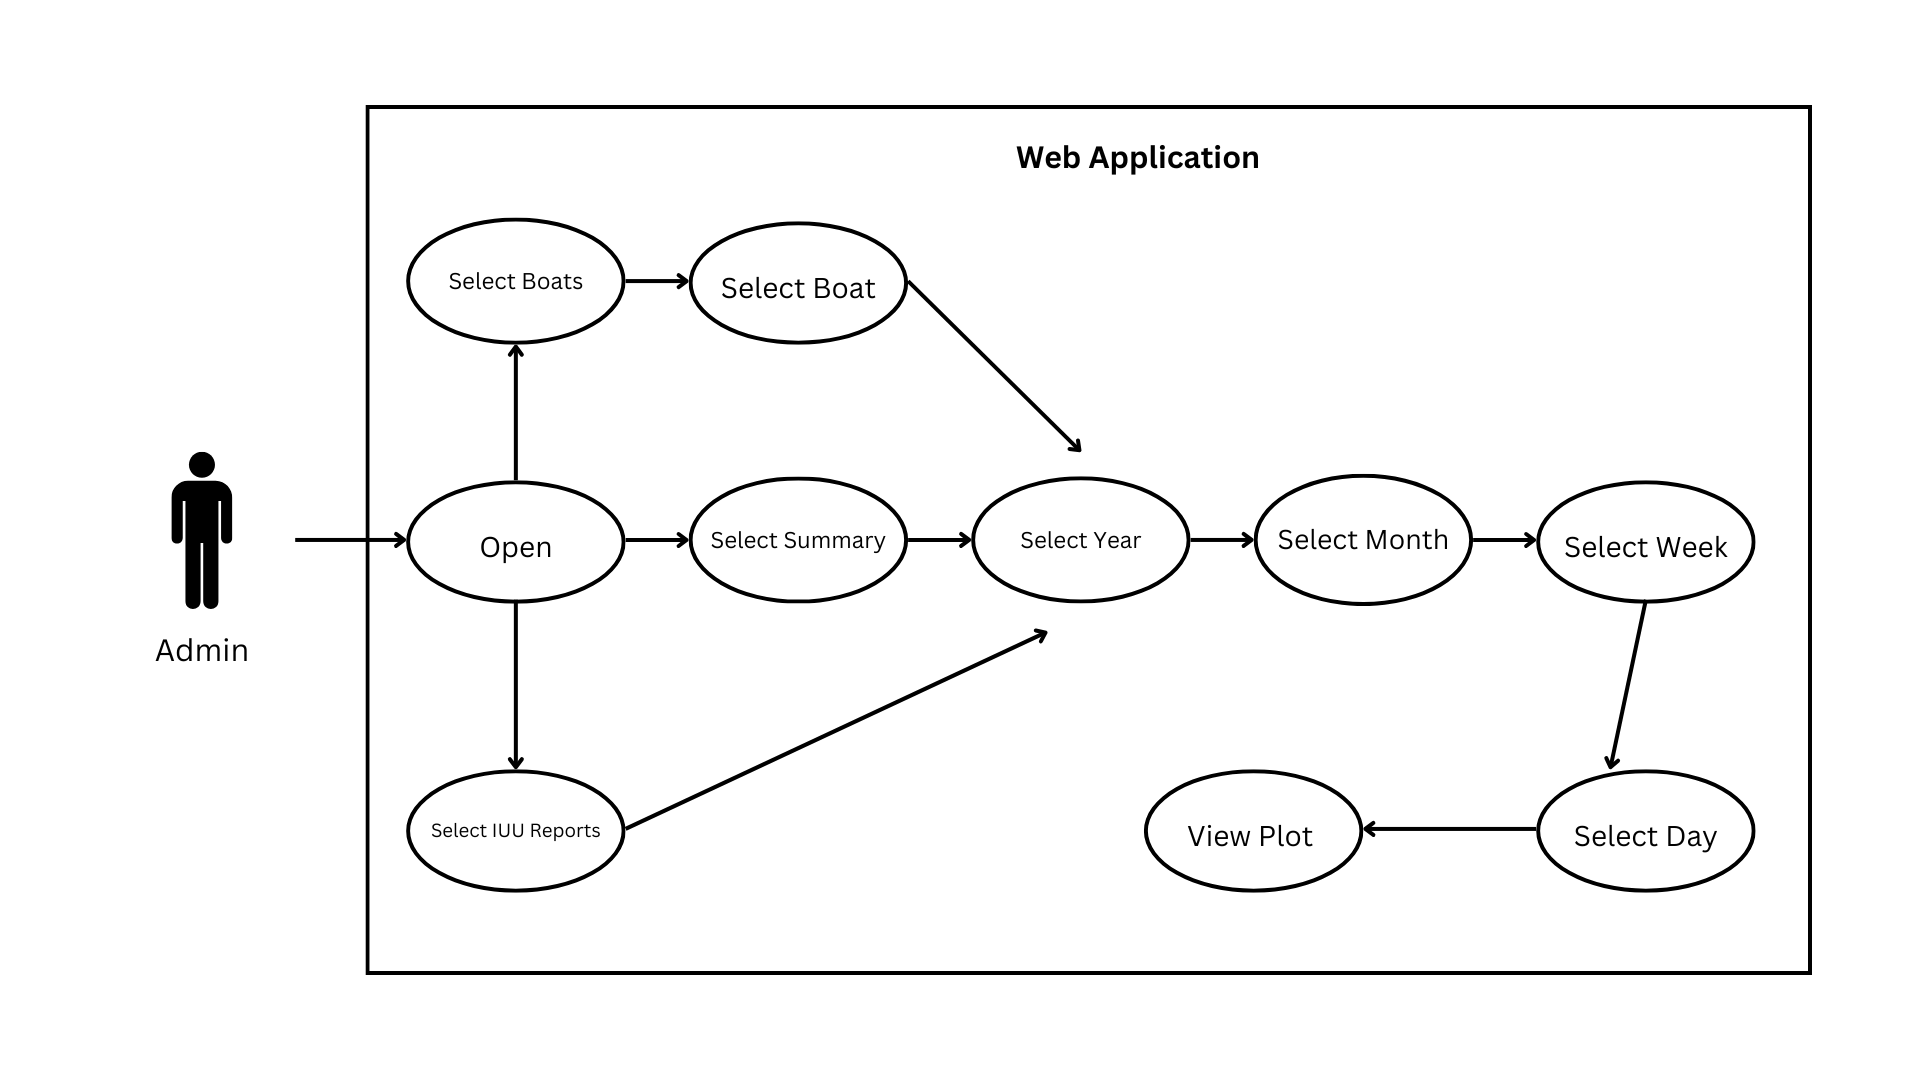
\includegraphics[width=1\linewidth]{Figure_2.png}
    \caption{Use Case Diagram for the Web Platform}
    \label{fig:enter-label}
\end{figure}


\subsection{System Overview}
The BantayLaot system integrates a mobile application and a web-based platform to enable comprehensive monitoring of fishing activities and violations. Both components interact with a centralized MongoDB database managed through a Node.js server. The system architecture ensures seamless data synchronization and visualization.

\subsection{Mobile Application Features}
The mobile application serves as a primary tool for data collection, designed for use by fishermen in the field. Key features include:
\begin{itemize}
    \item \textbf{Location Tracking:} Utilizes GPS data to record fishing routes, encoded with timestamps for spatial-temporal analysis.
    \item \textbf{Fishing Session Reports:} Allows users to log fishing activities, including gear types, species caught, and total catch weight.
    \item \textbf{Violation Reporting:} Supports the capture and upload of multimedia evidence (e.g., images) for IUU violations, which are automatically encoded into Base64 format for efficient transmission.
    \item \textbf{Offline Functionality:} Data is locally stored using SQLite via the Room persistence library and synced to MongoDB once an internet connection is re-established.
\end{itemize}

\subsection{Web Application Features}
The web platform is designed for data visualization and analysis. Its features include:
\begin{itemize}
    \item \textbf{Geospatial Visualization:} Displays fishing sessions and IUU violations on an interactive map using \texttt{OpenLayers}.
    \item \textbf{Data Summarization:} Provides aggregated metrics, including Catch Per Unit Effort (CPUE), via dynamic charts.
    \item \textbf{Violation Analytics:} Offers detailed summaries and filtering options for IUU violations, enabling temporal and spatial trend analysis.
    \item \textbf{Boat-Specific Insights:} Facilitates the examination of data per vessel, including activity summaries and catch statistics.
\end{itemize}

\subsection{Data Collection}
The BantayLaot system collects essential data from municipal fisheries, focusing on fishing activities and reporting violations of fishing laws. The system categorizes collected information into two primary types: fishing-related data and IUU (Illegal, Unreported, and Unregulated) reporting data.

\subsubsection{Fishing Data}
The fishing data gathered provides comprehensive insights into the operations of municipal fishermen, supporting sustainable practices and fisheries management. The data includes:
\begin{enumerate}
    \item \textbf{Fishing Gear:} Types of fishing gear used during sessions.
    \item \textbf{Fish Catch Information:} Local fish species and corresponding catch weights.
    \item \textbf{Location Tracking:} GPS coordinates logged throughout fishing sessions.
    \item \textbf{Session Details:} Start and end timestamps of fishing activities.
\end{enumerate}

\subsubsection{IUU Reporting Data}
To combat IUU fishing, the system facilitates the reporting of violations directly from fishermen or other users. The reported data includes:
\begin{enumerate}
    \item \textbf{Violation Details:} Specific violations based on predefined categories.
    \item \textbf{Fishing Gear Involved:} Details of illegal or unauthorized fishing gear.
    \item \textbf{Violator Information:} Identifier of the violator and vessel.
    \item \textbf{Location of the Violation:} GPS coordinates of the incident.
    \item \textbf{Supporting Evidence:} Photos or multimedia evidence uploaded to substantiate the report.
\end{enumerate}

\section{Results and Discussion}
\label{sec:results}

\subsection{Mobile Application Implementation}
The mobile application was developed using Kotlin and Android Jetpack Compose for modern, responsive UI components. It is designed to function both online and offline, leveraging Room for local storage and GPSLocationService for accurate location tracking.

\subsubsection{Home Page}
The Home Page serves as the gateway to the app’s functionalities, including starting fishing sessions, reporting violations, and submitting catch data (Figure~\ref{fig:mobile-home}). 

\begin{figure} [H]%
    \centering
    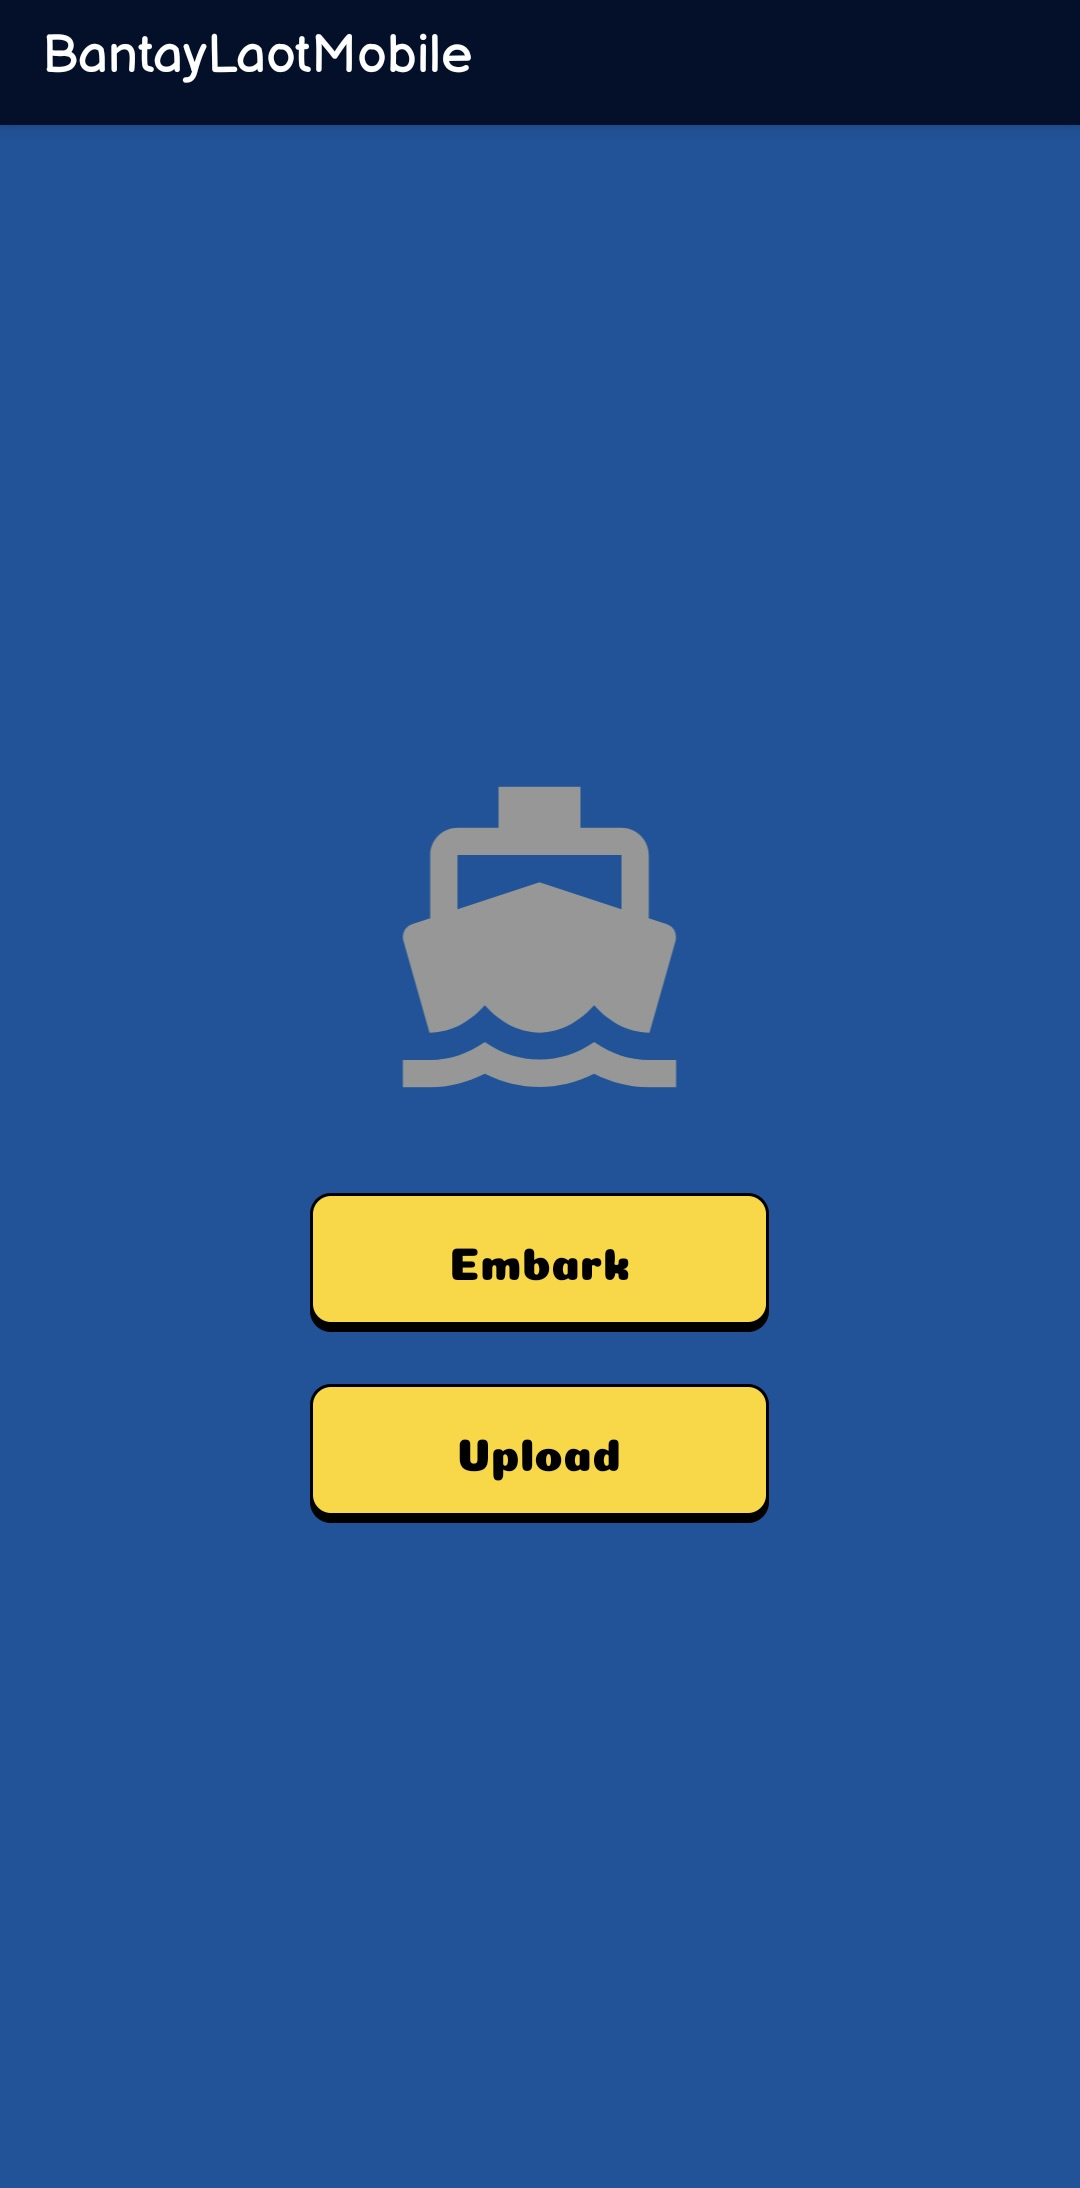
\includegraphics[width=0.4\linewidth]{Figure_5.jpeg}
    \caption{The Home Page}
    \label{fig:mobile-home}
\end{figure}

\subsubsection{GPS Tracking}
When a fishing session starts, the application records GPS data continuously, displaying elapsed time and coordinates in real-time (Figure~\ref{fig:mobile-gps}).

\begin{figure} [H]%
    \centering
    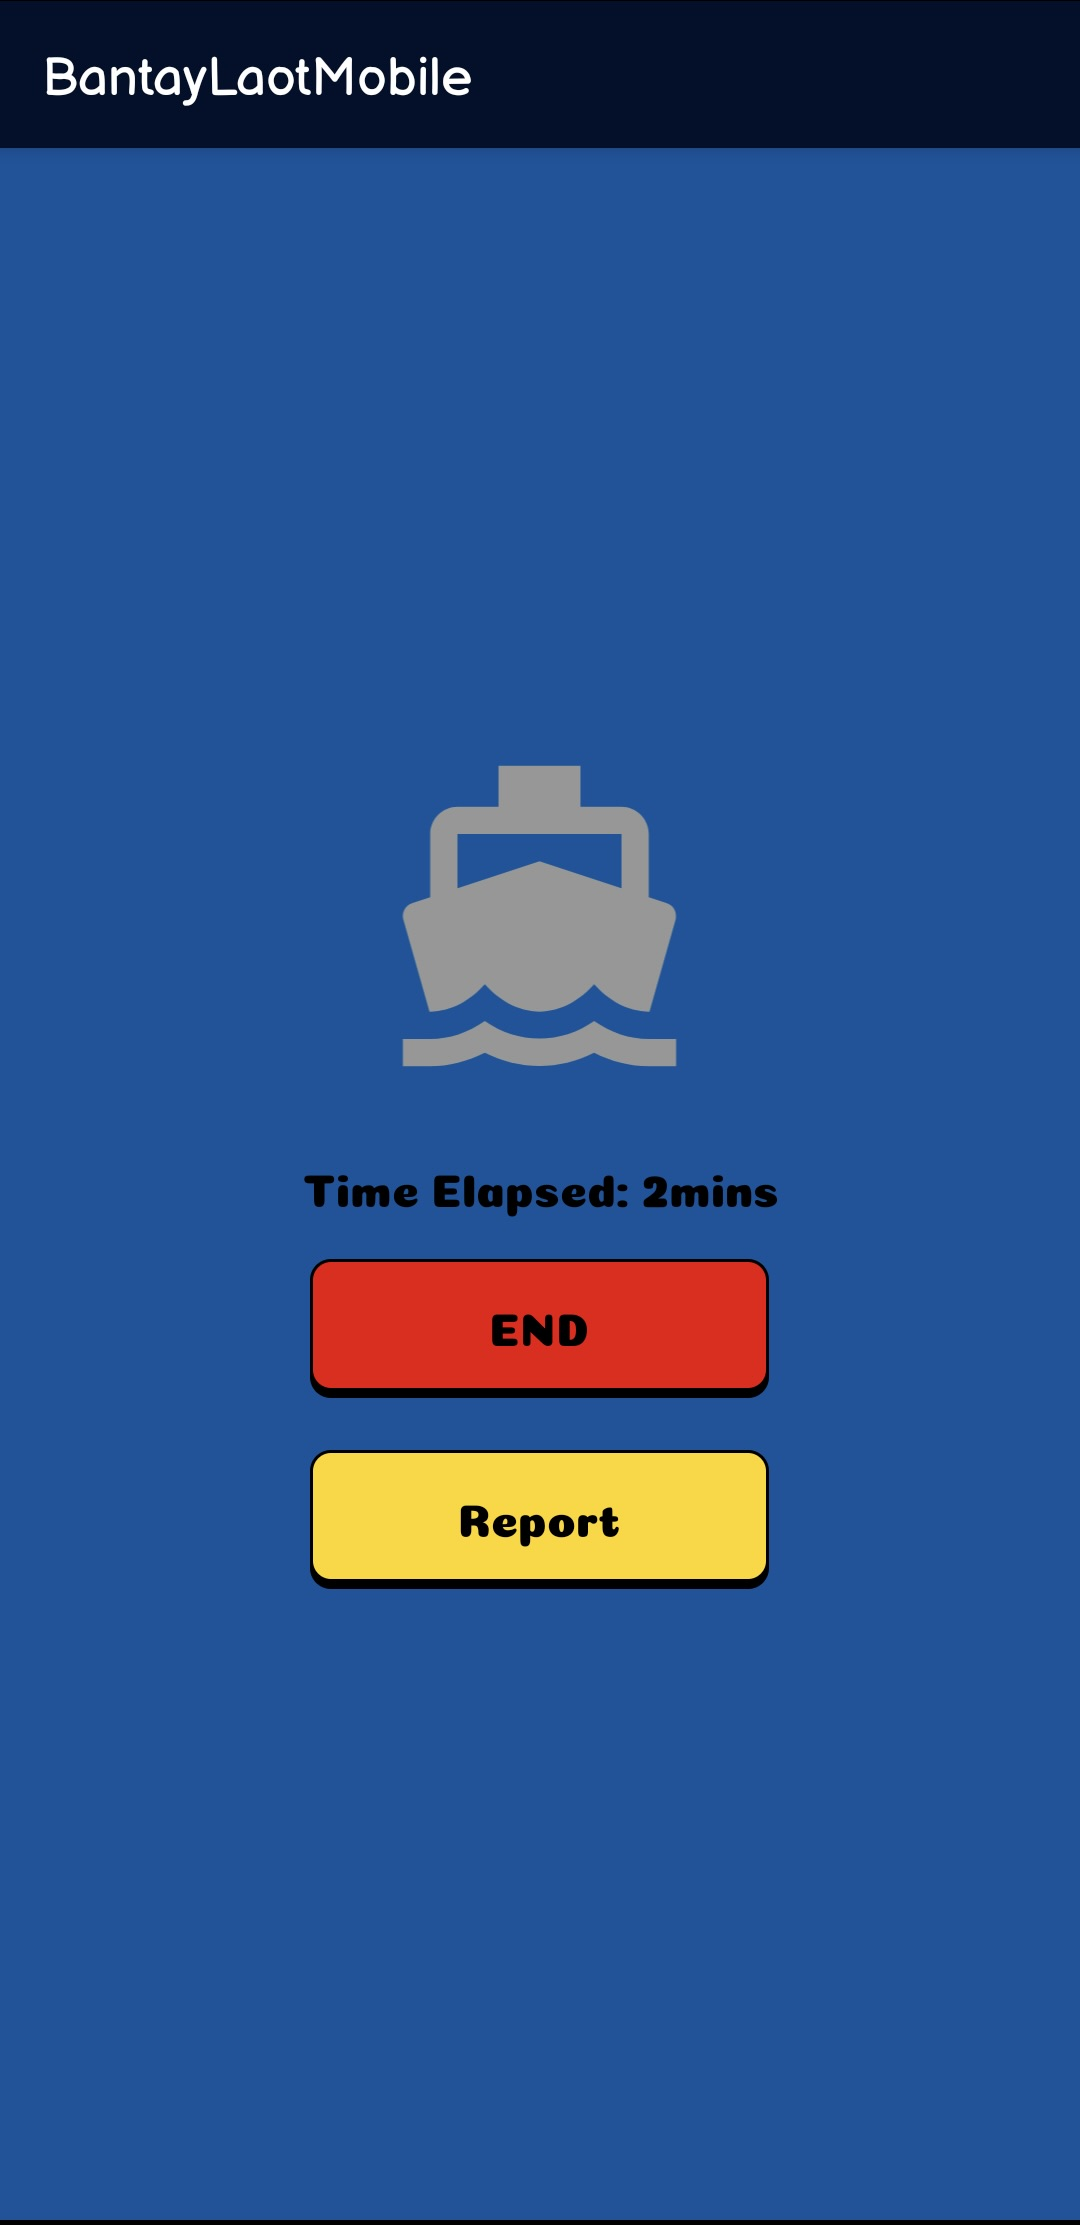
\includegraphics[width=0.4\linewidth]{Figure_6.jpeg}
    \caption{The view of the home page when a session is ongoing}
    \label{fig:mobile-gps}
\end{figure}

\subsubsection{Catch Reporting}
The catch reporting feature allows users to document their fish species, weights, and gear used. Users can add multiple entries for different types of fishing gear (Figure~\ref{fig:catch-reporting}).

\begin{figure} [H]%
    \centering
    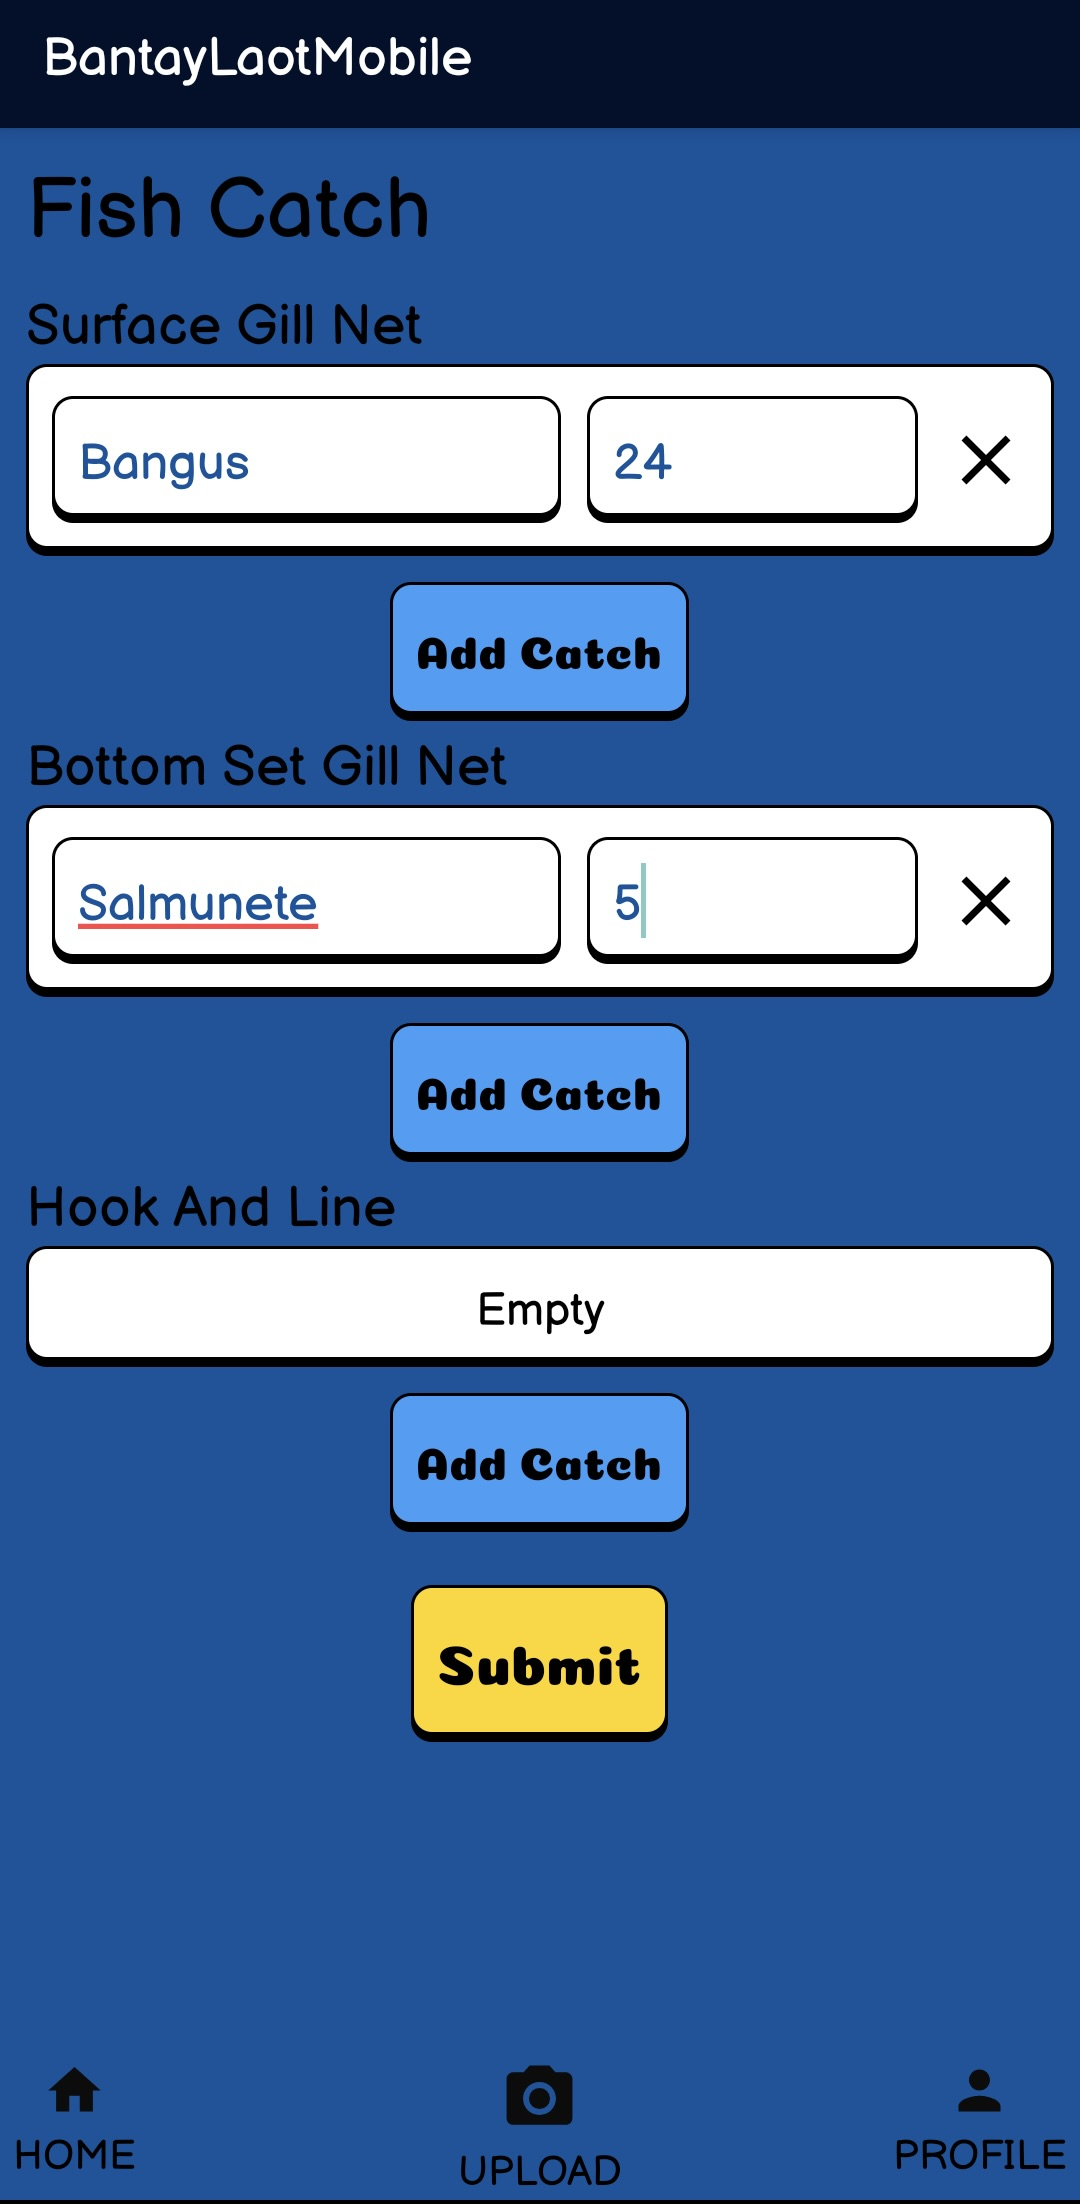
\includegraphics[width=0.4\linewidth]{Figure_7.jpeg}
    \caption{A filled in Fish Catch Documentation}
    \label{fig:catch-reporting}
\end{figure}

\subsubsection{Violation Reporting}
Violations can be reported using a dedicated form that captures details such as violator information, violation type, location, and supporting image evidence (Figure~\ref{fig:violation-reporting}).

\begin{figure} [H]%
    \centering
    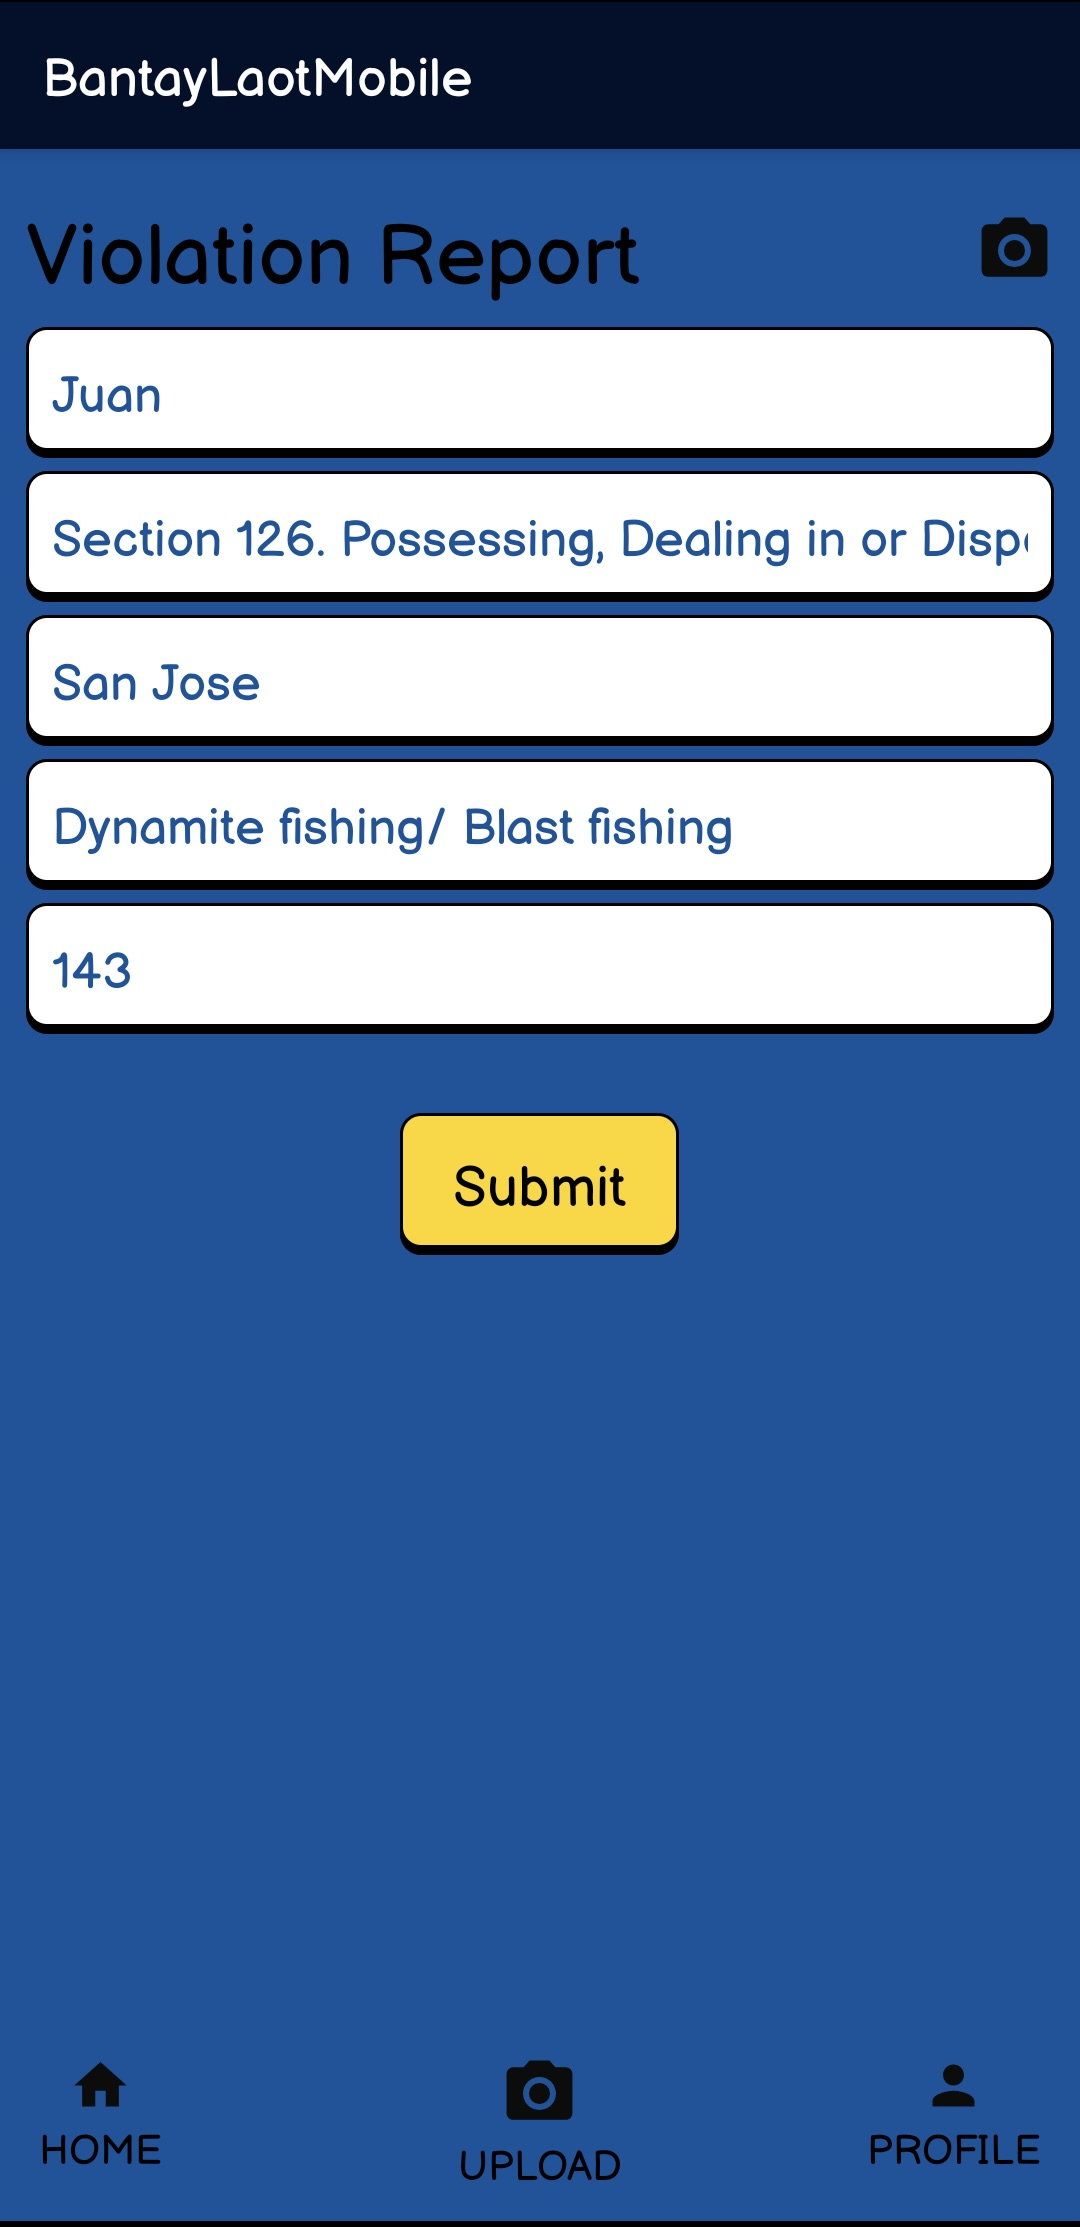
\includegraphics[width=0.4\linewidth]{Figure_8.jpeg}
    \caption{A filled in violation report}
    \label{fig:violation-reporting}
\end{figure}


\subsubsection{Offline Data Upload}
The app stores data locally when offline and syncs it to the backend once a connection is re-established. This ensures that the system is operational in areas with poor internet connectivity.

\subsection{Web Platform Implementation}
The web platform was built using the MERN stack (MongoDB, Express.js, React, and Node.js) and OpenLayers for interactive geospatial visualization. The platform provides stakeholders with tools to monitor fishing activities and violations.

\subsubsection{Dashboard}
The dashboard presents an overview of total fishing sessions, violations reported, and catch per unit effort (CPUE) metrics (Figure~\ref{fig:web-dashboard}).

\begin{figure} [H]%
    \centering
    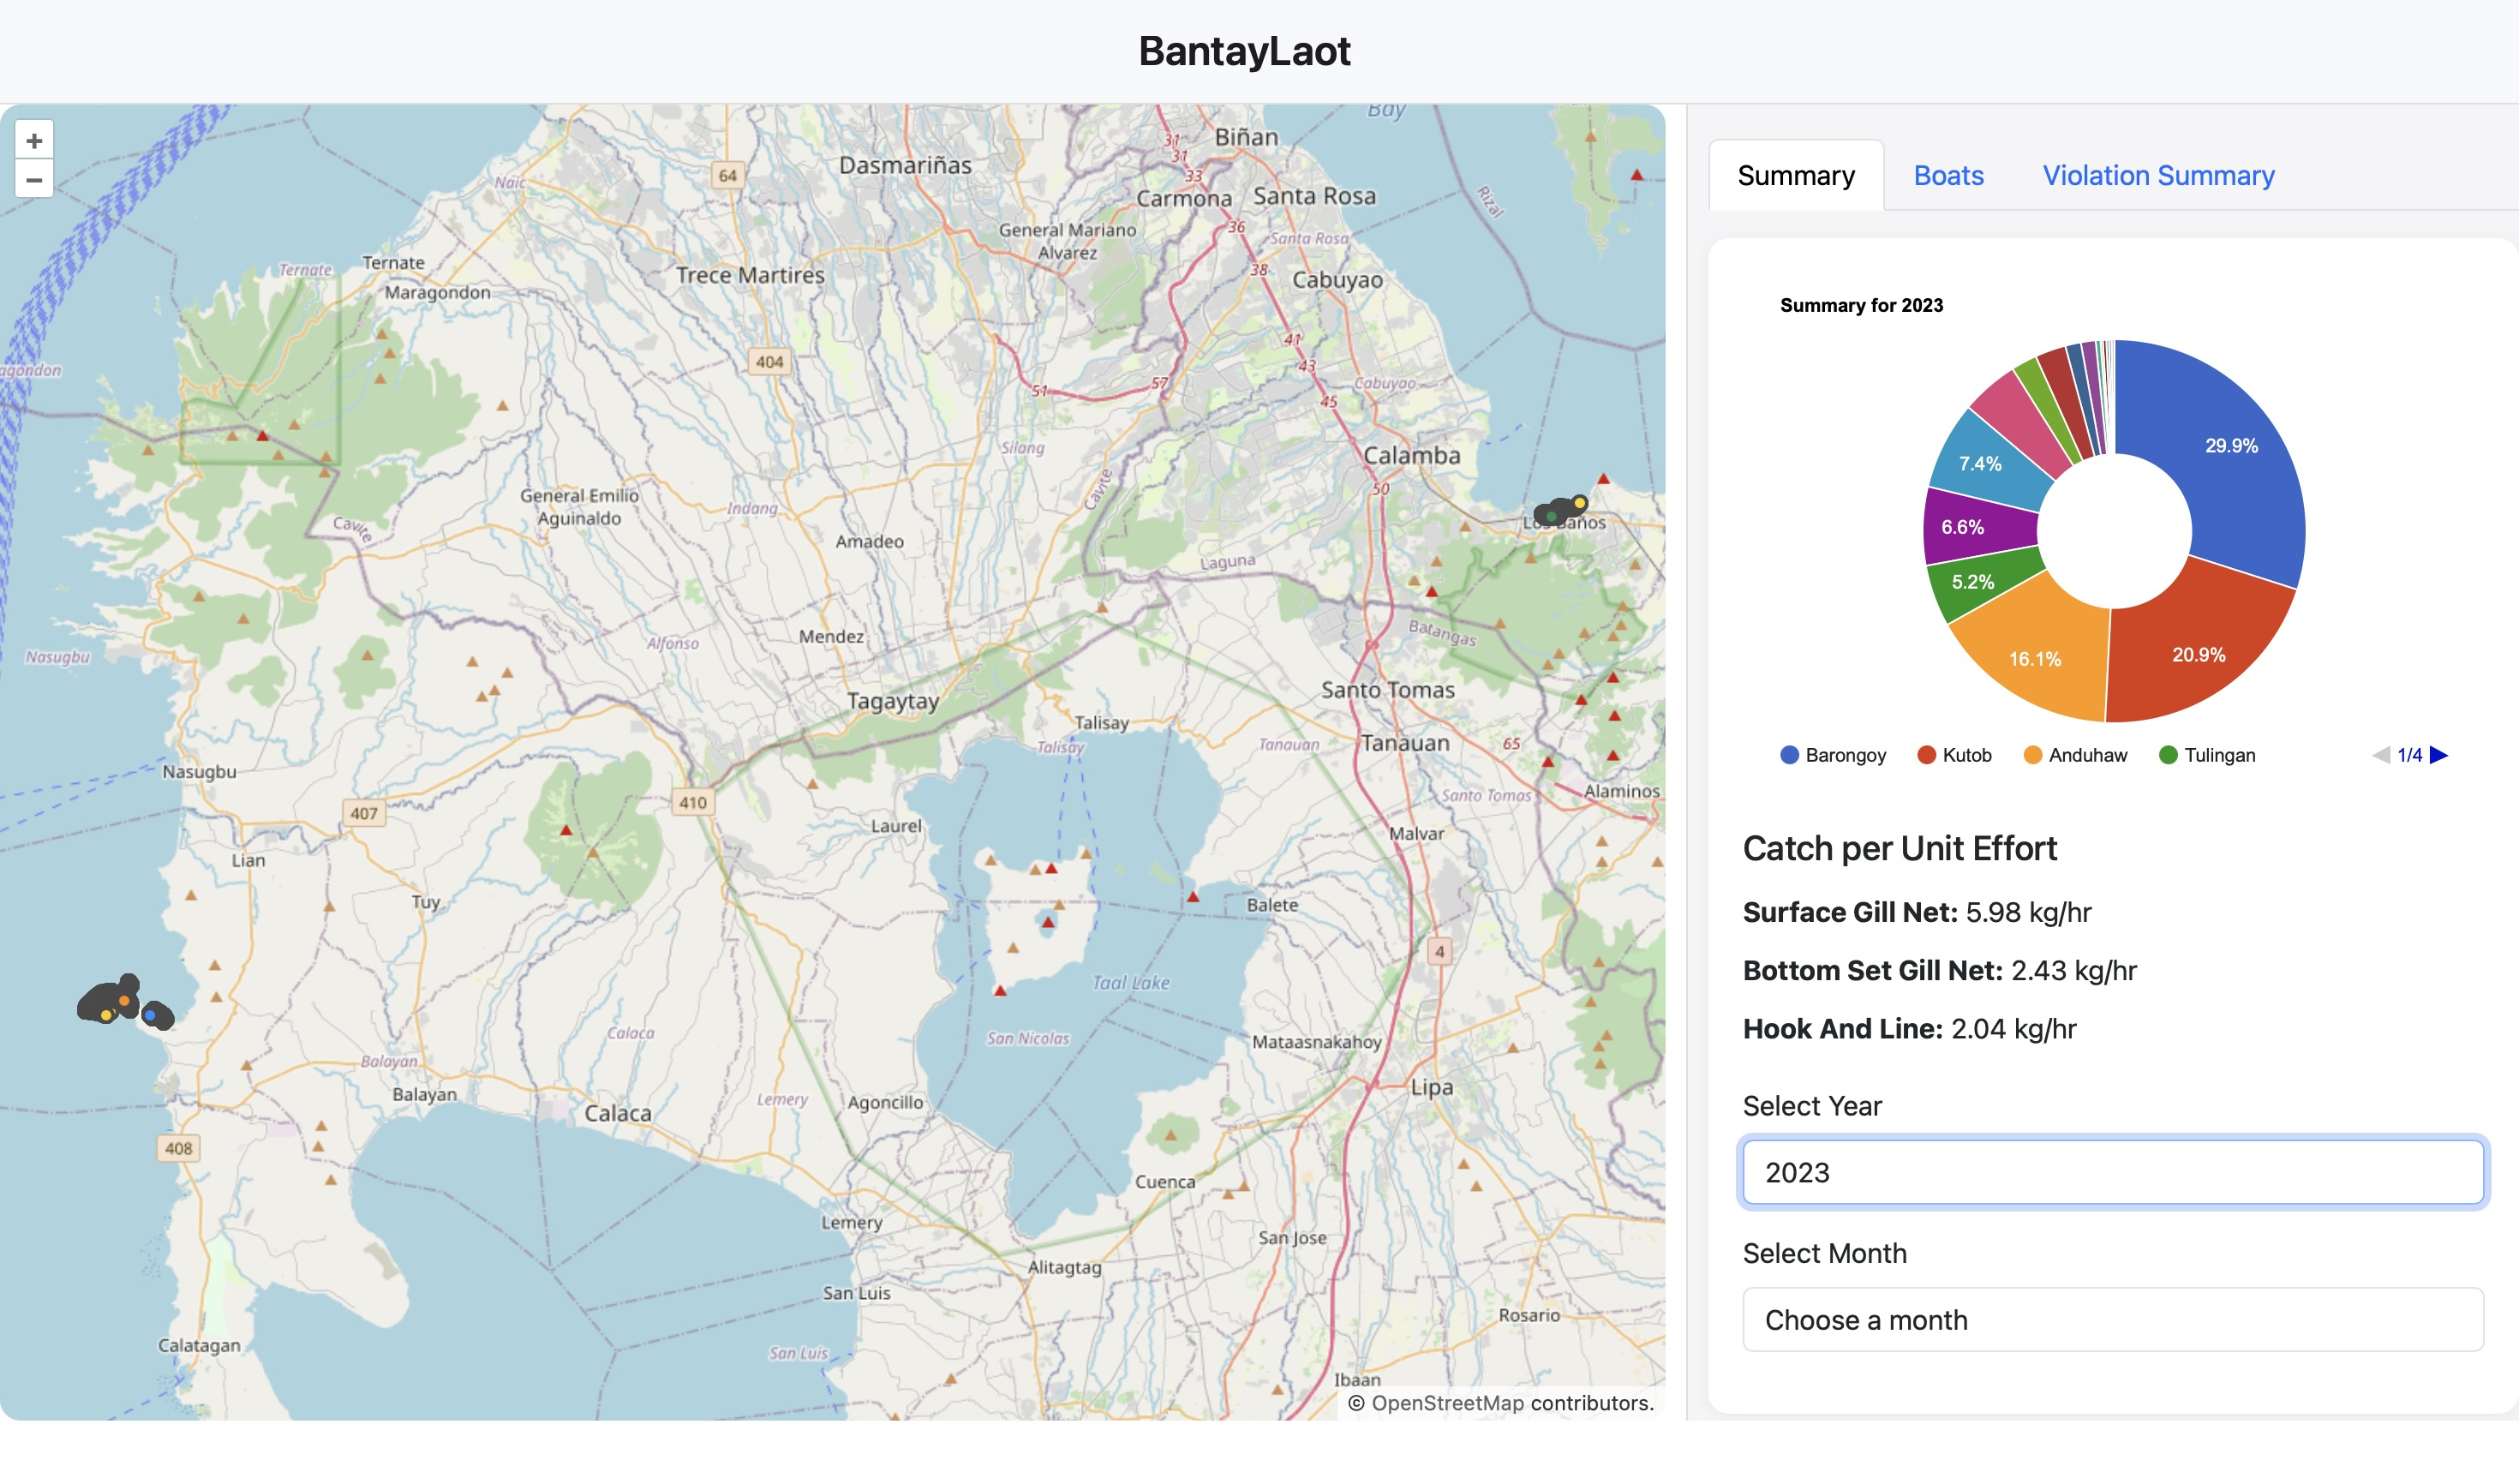
\includegraphics[width=0.9\linewidth]{Figure_9.jpeg}
    \caption{The dashboard}
    \label{fig:web-dashboard}
\end{figure}


\subsubsection{Interactive Map}
The interactive map visualizes fishing routes and IUU violations, with clickable markers providing detailed information (Figure~\ref{fig:interactive-map}).

\begin{figure} [H]%
    \centering
    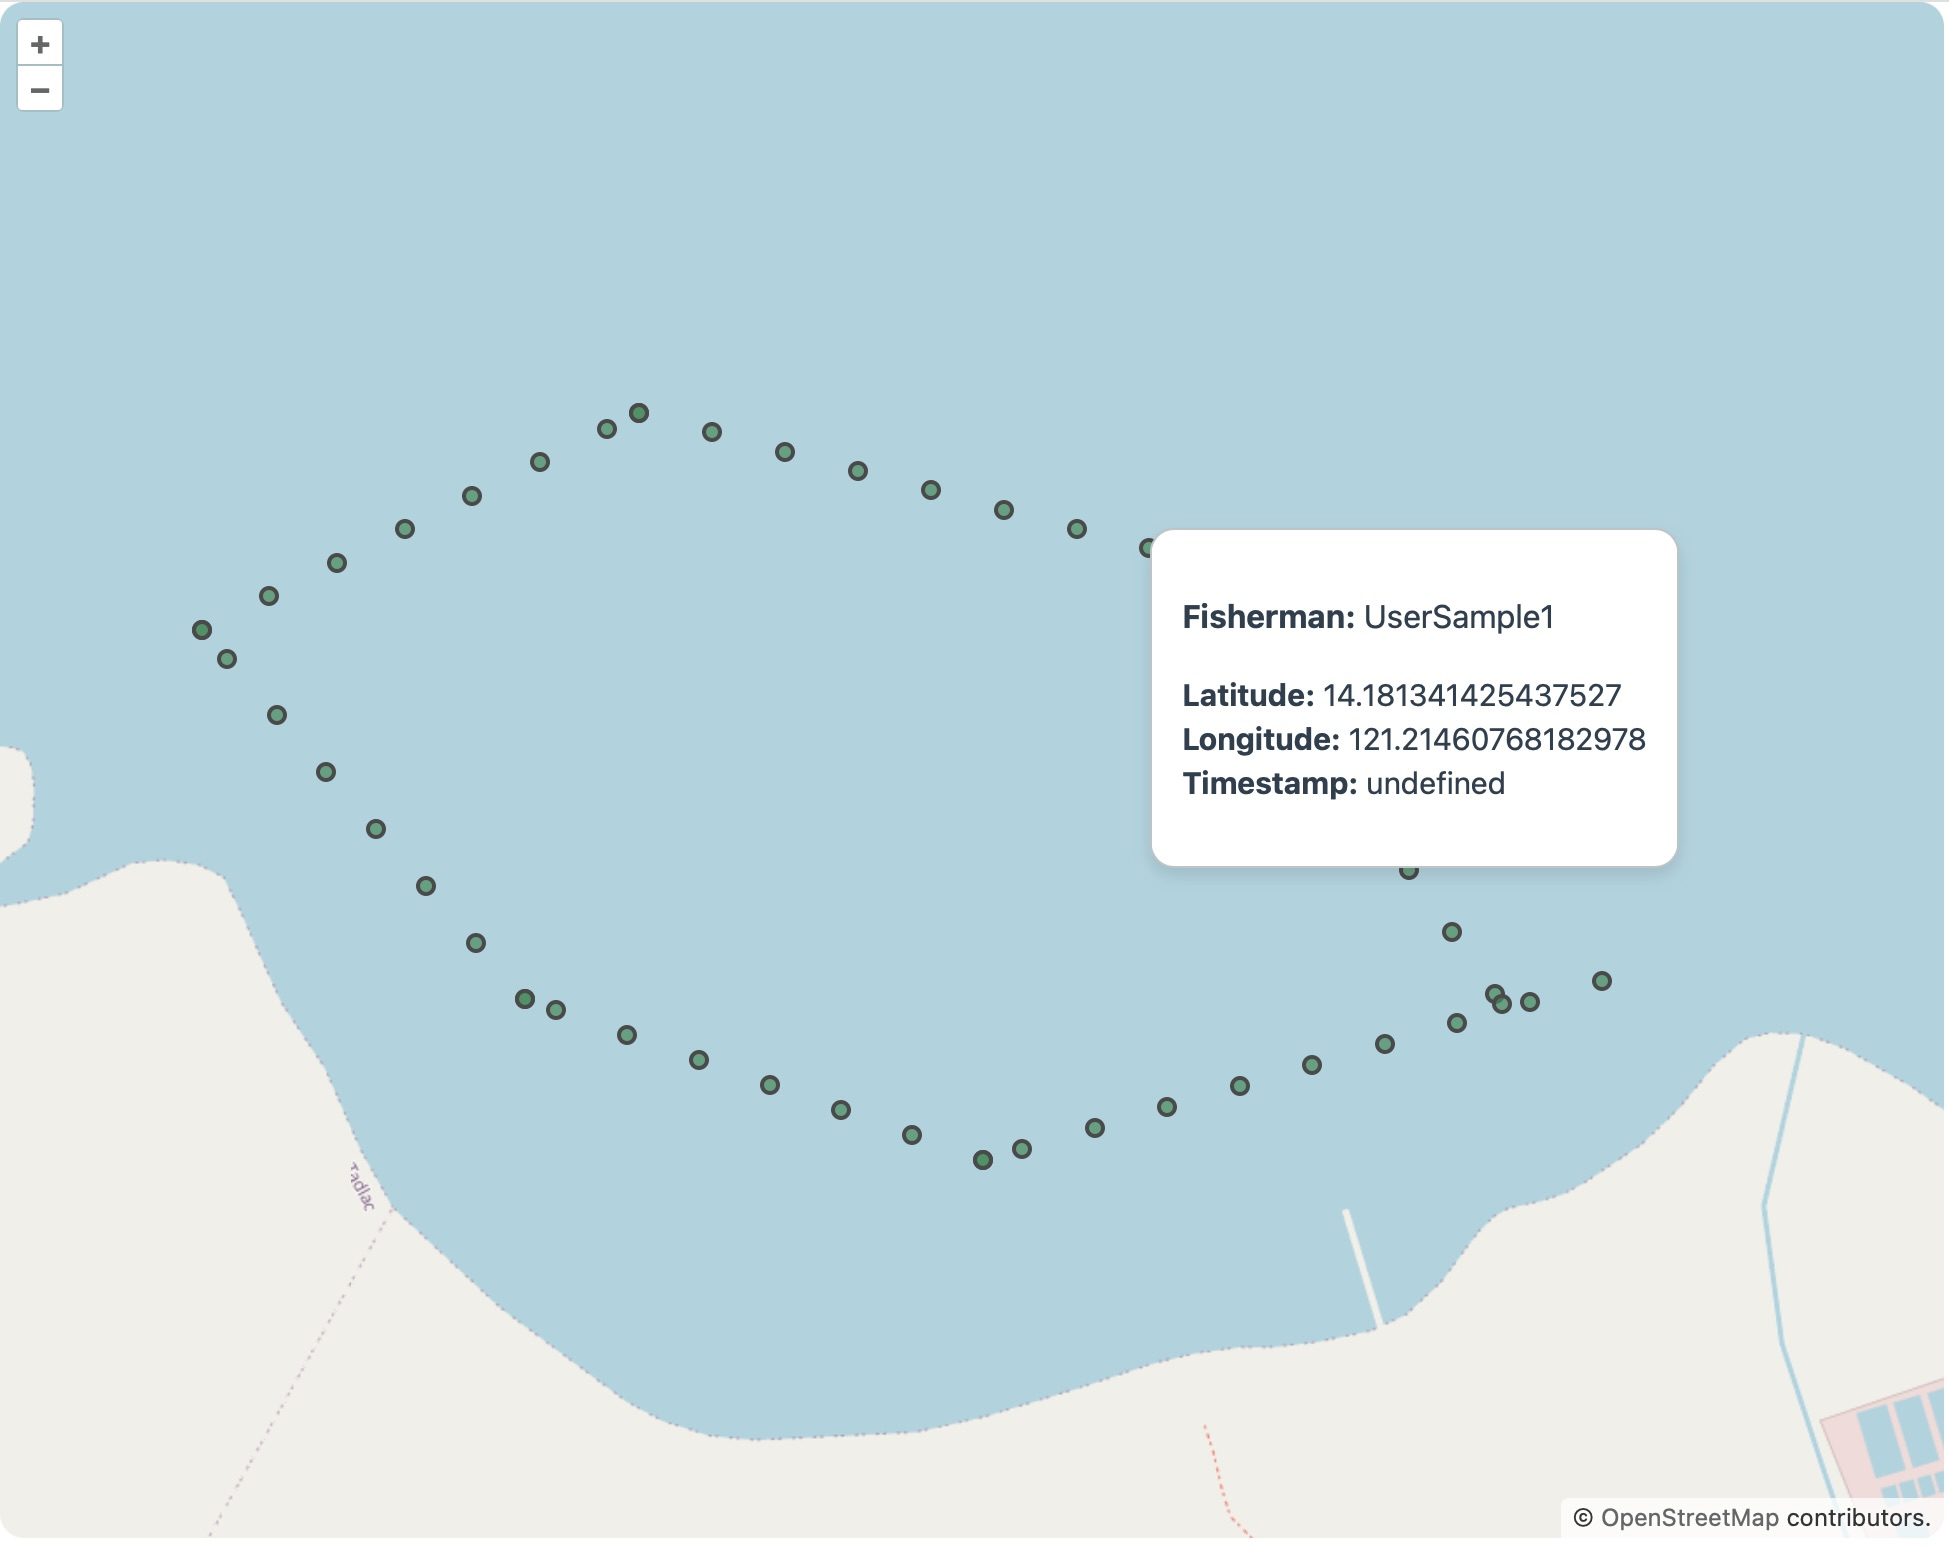
\includegraphics[width=0.85\linewidth]{Figure_10.jpeg}
    \caption{The interactive map with plots and details of the plot opened}
    \label{fig:interactive-map}
\end{figure}



\subsubsection{Violation Summary}
Violation trends are summarized in charts, enabling stakeholders to identify patterns and target enforcement efforts (Figure~\ref{fig:violation-summary}).

\begin{figure} [H]%
    \centering
    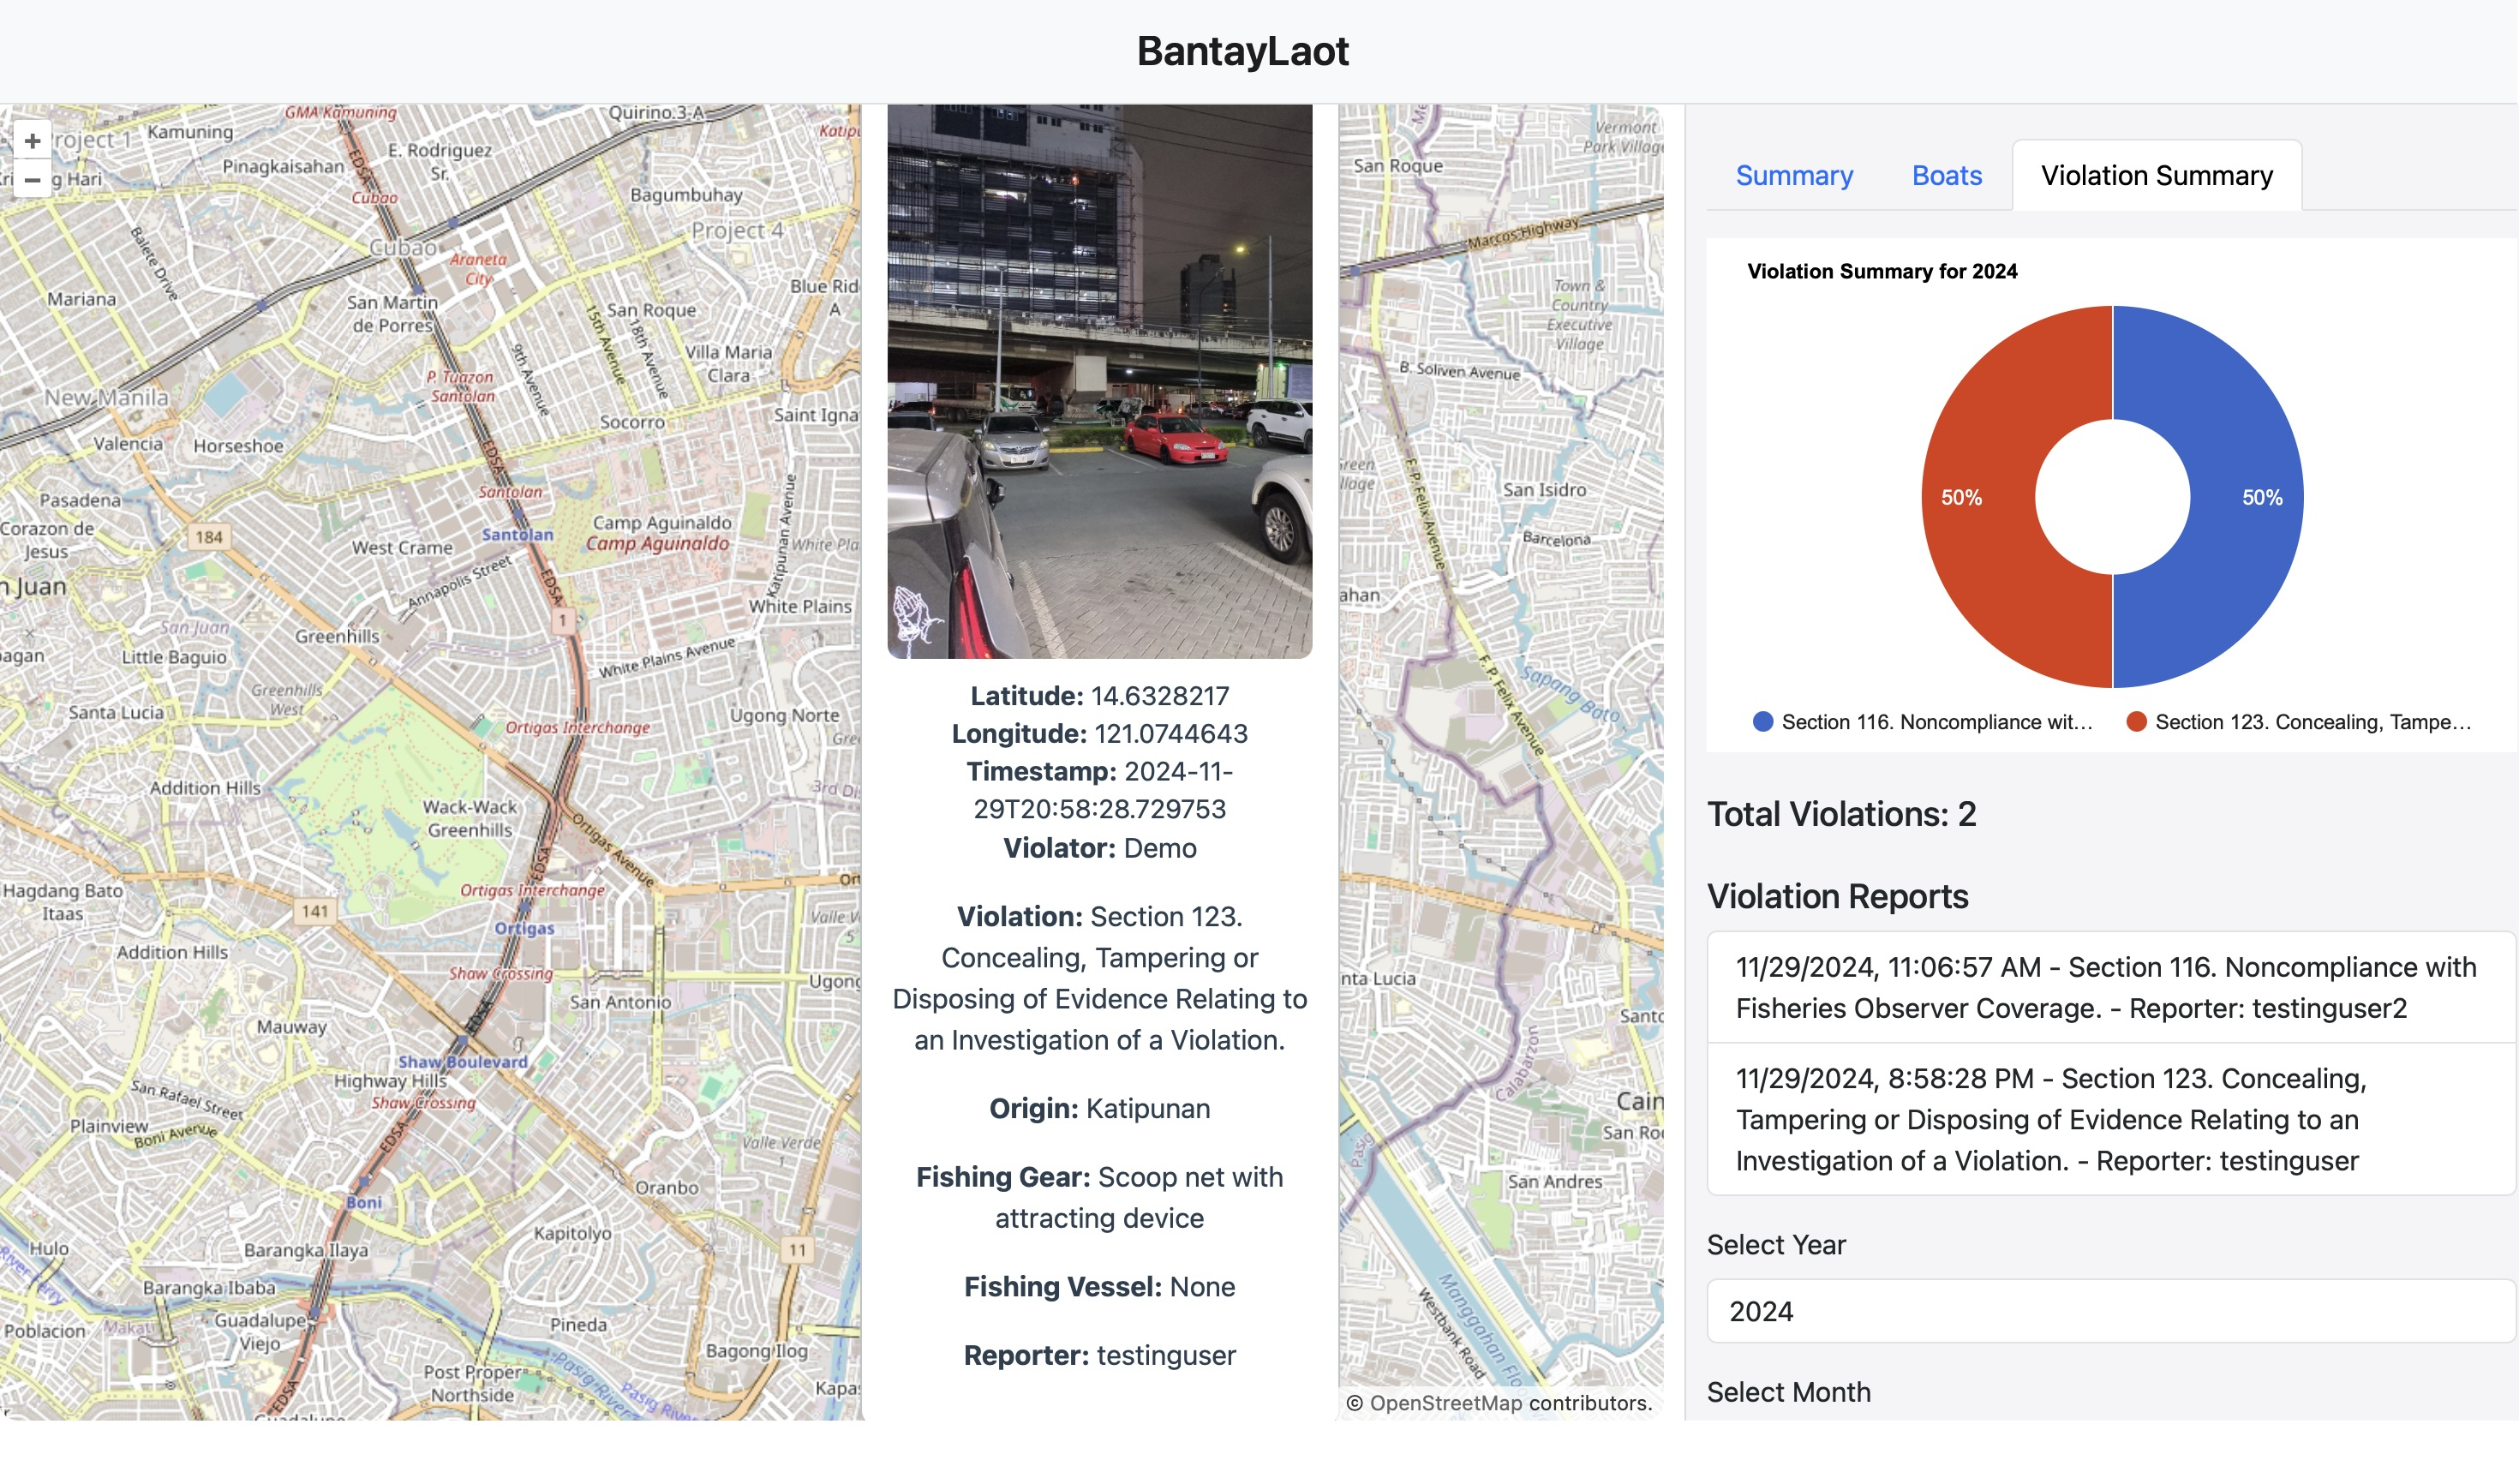
\includegraphics[width=0.9\linewidth]{Figure_11.jpeg}
    \caption{IUU details from plot and the IUU Report Tab}
    \label{fig:violation-summary}
\end{figure}



\subsubsection{Boat-Specific Metrics}
Analytics for individual boats include CPUE by gear type and fishing effort visualized through dynamic charts (Figure~\ref{fig:boat-metrics}).

\begin{figure} [H]%
    \centering
    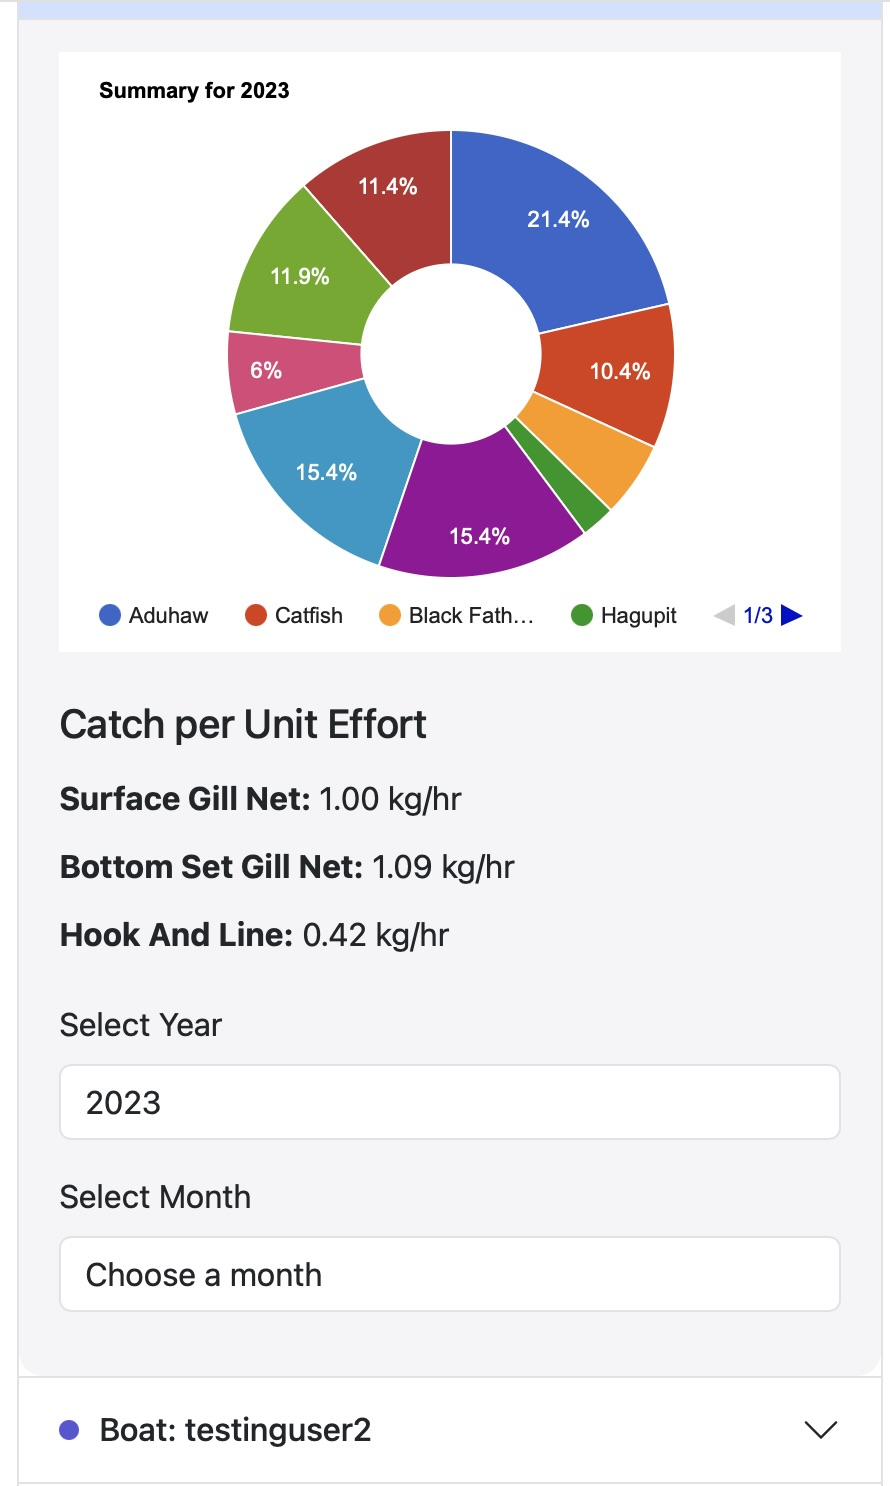
\includegraphics[width=0.5\linewidth]{Figure_12.jpeg}
    \caption{Fish catch summary and CPUE for each equipment of a boat}
    \label{fig:boat-metrics}
\end{figure}

\section{Conclusion and Recommendations}

\subsection{Conclusion}

The development and implementation of BantayLaot demonstrate the feasibility of using mobile and web technologies to address the challenges of illegal, unreported, and unregulated (IUU) fishing in the Philippines. The system successfully integrates GPS-based tracking, fish catch documentation, and a reporting mechanism for IUU fishing, with seamless data synchronization between the mobile application and the web platform.

While the system was not tested on actual fishing vessels, its functionality was validated through real-time testing on land, using walking and vehicle simulations. These tests confirmed the reliability of data collection, synchronization, and visualization processes. The mobile application effectively recorded and transmitted data, while the web platform displayed this information accurately through geospatial visualizations and summary charts. Additionally, the reporting system for violations worked as intended, allowing detailed information to be captured and displayed effectively.

Despite these achievements, the system's lack of field testing on water highlights the need for further validation to assess its performance in actual fishing conditions. Nonetheless, BantayLaot provides a robust foundation for improving municipal fisheries management, supporting sustainable practices, and addressing the socioeconomic challenges faced by coastal communities.

\subsection{Recommendations}

To further enhance the functionality and applicability of BantayLaot, several improvements are recommended. Field testing on municipal fishing vessels should be conducted to validate the system’s performance in real-world conditions and to gather feedback from its intended users. Implementing an account system will improve data security, allow personalized dashboards, and ensure better traceability of reports. The integration of image processing for fish recognition could automate the identification of fish species, reducing manual input and enhancing the accuracy of catch documentation. 

The mobile application’s offline functionality should also be optimized to handle prolonged periods of no internet connectivity, ensuring consistent performance in remote areas. Finally, integrating BantayLaot with government regulatory systems would enable real-time action on reported violations, further supporting sustainable fisheries management. These enhancements will address the limitations of the current implementation and maximize the system’s potential as a tool for combating IUU fishing in the Philippines.

\section*{Acknowledgments}
I would like to express my deepest gratitude to my adviser, Dr. Val Randolf M. Madrid, for his invaluable guidance, support, and encouragement throughout the course of this research. His expertise and insights have been instrumental in the completion of this study.

I am profoundly thankful to my mother and siblings for their unconditional love, support, and sacrifices, which have been a constant source of inspiration and strength.

A special acknowledgment goes to my girlfriend, Alexandra B. Brigino, for her unwavering patience, understanding, and encouragement during the challenging moments of this journey.

Finally, I wish to thank my brothers at The Corvus for their camaraderie, support, and for fostering an environment that promotes academic excellence and personal growth, successus unius triumphus omnium.


\ifCLASSOPTIONcaptionsoff
  \newpage
\fi

\newpage

\begin{thebibliography}{11}

\bibitem{Ardito2020}
L. Ardito, R. Coppola, G. Malnati, and M. Torchiano, ``Effectiveness of Kotlin vs. Java in android app development tasks,'' \emph{Information and Software Technology}, vol. 127, 2020. [Online]. Available: https://doi.org/10.1016/j.infsof.2020.106374.

\bibitem{Baid2024}
J. Baid and S. Gupta, ``COMPARATIVE ANALYSIS OF MERN, MEAN AND MEVN STACKS IN WEB DEVELOPMENT,'' \emph{INTERANTIONAL JOURNAL OF SCIENTIFIC RESEARCH IN ENGINEERING AND MANAGEMENT}, vol. 08, no. 02, pp. 1–10, 2024. [Online]. Available: https://doi.org/10.55041/ijsrem28539.

\bibitem{Bawane2022} M. Bawane, I. Gawande, V. Joshi, R. Nikam, and S. A. Bachwani, "A Review on Technologies Used in MERN Stack," \emph{International Journal for Research in Applied Science \& Engineering Technology (IJRASET)}, vol. 10, no. 1, pp. 479–488, January 2022. DOI: 10.22214/ijraset.2022.39868.

\bibitem{Calderwood2022}
J. Calderwood, ``Smartphone application use in commercial wild capture fisheries,'' \emph{Reviews in Fish Biology and Fisheries}, vol. 32, no. 4, pp. 1063-1083, 2022.

\bibitem{Coastal2021}
Coastal Resources Center, ``Quantifying the Prevalence and Impact of Illegal, Unreported and Unregulated Fishing in the Philippines Workshop Report,'' USAID Fish Right Program, Narragansett, RI, 2021.

\bibitem{Fotache2013}
M. Fotache and D. Cogean, ``NoSQL and SQL Databases for Mobile Applications. Case Study: MongoDB versus PostgreSQL,'' \emph{Informatica Economica}, vol. 17, no. 2, pp. 41–58, 2013. [Online]. Available: https://doi.org/10.12948/issn14531305/17.2.2013.04.

\bibitem{Gerritsen2011}
H. Gerritsen and C. Lordan, ``Integrating vessel monitoring systems (VMS) data with daily catch data from logbooks to explore the spatial distribution of catch and effort at high resolution,'' \emph{ICES Journal of Marine Science}, vol. 68, no. 1, pp. 245–252, 2011. [Online]. Available: https://doi.org/10.1093/icesjms/fsq137.

\bibitem{Hussain2021}
H. Hussain, K. Khan, F. Farooqui, Q. Ali Arain, and I. Farah Siddiqui, ``Comparative Study of Android Native and Flutter App Development,'' \emph{Memory}, vol. 47, pp. 36–37, 2021.

\bibitem{PSA2023}
Philippine Statistics Authority, ``Official Poverty Statistics among Basic Sectors in the Philippines,'' 2023. [Online]. Available: https://www.psa.gov.ph/content/fisherfolks-and-farmers-remain-have-highest-poverty-incidences-among-basic-sectors-2021.

\bibitem{Soemarmi2020}
A. Soemarmi, E. Indarti, P. Wardhani, L. T. A. L., A. Diamantina, and A. Ristyawati, ``The use of the vessel monitoring system as fishery ship obligations in indonesia,'' \emph{AACL Bioflux}, vol. 13, no. 3, pp. 1483–1494, 2020.

\bibitem{Wahab2021}
A. Wahab, B. Waseso, and H. Pranoto, ``Synchronization of Catch Fish Data in Fisheries e-Logbook with a Vessel Monitoring System,'' \emph{International Journal of Advanced Technology in Mechanical, Mechatronics and Materials}, vol. 2, no. 1, pp. 46–54, 2021. [Online]. Available: https://doi.org/10.37869/ijatec.v2i1.43.

\end{thebibliography}

\begin{IEEEbiography}[{
\includegraphics[width=1.5in,height=1.3in,clip,keepaspectratio]{profile.jpeg}}]{Jose Benjamin Gallero} is a BS Computer Science Senior at the University of the Philippines Los Baños. Born in Sta. Maria, Bulacan and raised in Quezon City, Metro Manila, he is deeply passionate about Data Science. A former Chairperson of College of Arts and Student Council, member of the Young Software Engineers' Society, and a founding member of UP Internet Freedom Network and also of The Corvus, Benjie combines his expertise in technology and a strong dedication to leadership and empowerment of his colleagues.

\end{IEEEbiography}

\end{document}


